\graphicspath{{./images/algo}}
\section{Аналитическая часть}

\subsection{Экспортирование результата в таблицу}

Для построения таблицы температур было решено выбрать 27 точек (3x3x3).

\begin{figure}[H]
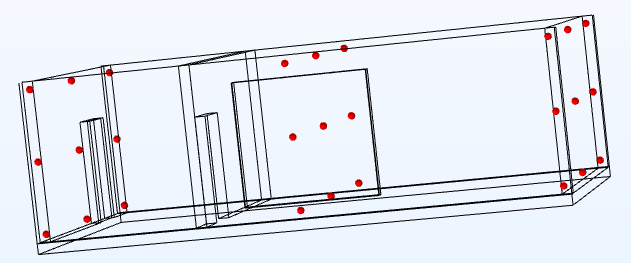
\includegraphics[width=\textwidth]{interesting_points.png}
\caption{27 points}
\end{figure}

Далее нужно уменьшить шаг с 1 часа до 5 минут. Сетка Normal с шагом 5 минут считалась 3 минуты, сетка Finer - 8 минут. 
Если выбрать сетку Coarse (более грубую, чем Normal), то расчет с шагом 30 секунд на протяжении суток занимает 11 минут.\\
Для выбора оптимального варианта по времени и качеству, нужно сравнить температуры в точках на шагах в 5 минут.
Для этого можно рассмотреть значения температур в некоторых точках при значении времени 86100 сек (5 минут до окончания расчета).
Для coarser значения в первых 5 точках:\\

\begin{table}[H]
\begin{tabular}{lllllll}
Mesh type  & Time  & (0.15, 0.15, 0.15) & (5, 0.15, 0.15) & (9.85, 0.15, 0.15) & (0.15, 3, 0.15) & (5, 3, 0.15) \\
Finer & 86100 & 307,57             & 305,54          & 296,95             & 308,44          & 297,94       \\
Coarse& 86100 & 306,17             & 299,38          & 296,72             & 308,11          & 298,29       \\ 
\end{tabular}
\end{table}
Можно видеть, что в некоторых точках значения могут отличаться на 5 градусов, что достаточно большая погрешность. Скорее всего связано это с тем, что внешняя часть стен была нагрета солнцем, поэтому имеет большую температуру, а из-за грубости сетки эта температура была передана и внутренней части, в которой находиться точка.\\
Поэтому варианты либо уменьшить сетку и пожертвовать временем (увеличить длительность вычислений или увеличить временной шаг), либо рассматривать точки на некотором расстоянии от стен

\newpage


\subsection{Критерий оптимальности точки}

\subsection{Предсказание температуры}
